\PassOptionsToPackage{quiet}{xeCJK}
\documentclass[UTF8,a4paper]{ctexart}
\usepackage[text={165mm,245mm}]{geometry}
\usepackage{graphicx}
\usepackage{subfigure}
\usepackage{ctex}
\usepackage{float} 
\usepackage{listings}
\usepackage{xcolor}
\usepackage{amsmath}
\usepackage{hyperref}
\usepackage{listings}
\newcommand{\code}{\texttt}
\graphicspath{{./img/}}
\definecolor{mygreen}{rgb}{0,0.6,0}  
\definecolor{mygray}{rgb}{0.5,0.5,0.5}  
\definecolor{mymauve}{rgb}{0.58,0,0.82}  


\title{\textbf{x-Eris 调研报告}}
\author{小组成员:胡天羽,罗胤玻,李润时,万辰希,吴书让}
\begin{document}
\maketitle

\section{项目概述}
随着嵌入式设备的存储空间容量也不断上升,原先的通过直接对指定地址写入数据的交互方式不再可行。因此,嵌入式系统需要有统一的文件系统来简化数据的存储组织方式。FreeRTOS是目前使用率最高的嵌入式系统之一,但是其文件系统并不完善。本项目旨在基于现有的FreeRTOS的虚拟文件系统模块FreeRTOS-Plus-Fat进行兼容性拓展及安全性能优化。
我们的项目计划实现以下特性:
\begin{itemize}
    \item 更好的兼容性
    \item 更高的性能
    \item 更好的安全性
\end{itemize}

我们将注重高性能的特点,例如目前大多数的文件系统仅支持基础功能,可以考虑通过添加缓存机制来优化性能。同时,文件系统的安全问题也很少被考虑到,可以通过加密算法、备份存储、读写权限等机制来增强文件系统的文件安全性。

我们计划从简单开始逐步完善项目,先扩展支持的文件系统,然后优化性能和安全性,最终视情况考虑对MMU的支持,分三步创建一个完整高效的文件系统。通过此项目,我们的目标是增强操作系统相关理论概念的理解,并掌握操作系统设计的能力。

\section{项目背景}
\subsection{物联网操作系统}
\subsubsection{概述}
物联网操作系统是指以操作系统内核(可以是 RTOS、Linux 等)为基础,包括如文件系统、图形库等较为完整的中间件组件,具备低功耗、安全、通信协议支持和云端连接能力的软件平台。

与传统的嵌入式设备相比,物联网感知层的设备更小、功耗更低,还需要安全性及组网能力,物联网通信层需要支持各种通信协议核协议之间的转换,应用层则需要具备云计算能力。在软件方面,支撑物联网设备的软件比传统的嵌入式设备软件更加复杂,这也对嵌入式操作系统提出了更高的要求。为了应对这种要求,一种面向物联网设备和应用的软件系统——物联网操作系统。

物联网中的操作系统涉及到芯片层、终端层、边缘层、云端层等多个层面.单一层次的物联网操作系统与安卓在移动互联网领域的地位和作用类似,实现了应用软件与智能终端硬件的解耦。就像在安卓的生态环境中,开发者基本不用考虑智能终端的物理硬件配置,只需根据安卓的编程接口编写应用程序,就可以运行在所有基于安卓的智能终端上一样,物联网操作系统的作用也是如此。

目前,物联网操作系统主要分为两大类,一是由传统的嵌入式实时操作系统(RTOS)发展而来,比如FreeRTOS、LiteOS、RT-Thread;二是由互联网公司的云平台延伸而来,基于传统操作系统进行“剪裁”和定制的IoT OS,比如Ali OS Things、TencentOS tiny、Win10 IOT。以下仅讨论已开源且有可行性的操作系统。

\subsubsection{\texttt{FreeRTOS}}
\begin{itemize}
\item 简介

FreeRTOS是与世界领先的芯片公司合作开发的,历时15年,是市场领先的微控制器和小型微处理器实时操作系统(RTOS)。FreeRTOS在MIT开源许可证下免费分发,包括一个内核和一组不断增长的物联网库,适用于所有行业。FreeRTOS的构建注重可靠性和易用性。FreeRTOS内核具有健壮性、占地面积小和广泛的设备支持,被世界领先的公司视为微控制器和小型微处理器的实际标准。预置演示项目和物联网 (IoT) 参考集成内容详尽,使使用者无需确定如何设置项目,能够快速下载、编译。其生态系统提供了广泛的选择,包括社区贡献和专业支持。

\item 优点
\begin{itemize}
    \item 具有实时性和可靠性等特点。
    \item 支持多种处理器架构和无线技术。
    \item 提供了一系列的驱动程序和库,如:FreeRTOS-Plus-TCP,FreeRTOS-Plus-CLI,FreeRTOS-Plus-FAT...   
\end{itemize}
\item 缺点
\begin{itemize}
    \item 不支持完整的文件系统,需要额外的第三方库支持。
    \item 对于处理大量数据和复杂任务的应用程序来说,可能存在性能瓶颈。     
\end{itemize}
\item 主要功能

任务管理、时间管理、信号量、消息队列、内存管理、记录功能、软件定时器、协程等,可基本满足较小系统的需要。
\item 语言

C和汇编, 其中绝大部分都是用C语言编写的,只有极少数的与处理器密切相关的部分代码才是用汇编写的。
\item 已支持的文件系统

主要为FAT文件系统
\item 相关库

FreeRTOS-Plus-FAT 是一种开源、线程感知和可扩展的 FAT12/FAT16/FAT32 DOS/Windows 兼容 嵌入式 FAT 文件系统,可支持全面线程感知、可扩展、支持 FAT12、FAT16 和 FAT32、明确到任务的工作目录、额外综合错误报告标准、全面的 API等功能。
\end{itemize}
\subsubsection{\texttt{RT-thread}}
\begin{itemize}
\item 简介

RT Thread是一个物联网平台,拥有丰富的中间层组件和强大的软硬件生态系统,几乎拥有物联网设备所需的所有关键基本组件,如网络协议、文件系统、低功耗管理等。它支持GCC等所有主流编译工具,使用统一的接口访问硬件外围设备。该系统可以自动进入睡眠模式,并支持动态电压和频率缩放。支持哈希、对称、gcm等算法,安全可靠,支持加密、防篡改、断点恢复、智能恢复、回溯等机制。动态模块和内核可以单独编译,在运行时,编译后的动态模块加载到内核中运行。遵循高度可重用的软件设计原则,一次性编程,永久使用。

\item 优点
\begin{itemize}
    \item 面向物联网设备:拥有跨芯片平台、实时操作系统内核、云端一体化、超低功耗设计等等
    \item 稳定可靠:已在工业界广泛应用
    \item 组件丰富:设备虚拟文件系统为应用提供统一的访问接口,支持FAT、UFFS、NFSv3、ROMFS等;轻型流媒体音频框架,支持常用音频格式,流媒体协议和DLNA/AirPlay...
    \item 简单易用:内置Shell调试工具,方便实时监测内核信息;UI Builder,配置器,包管理器等降低开发门槛,提升开发效率...
\end{itemize}
\item 主要功能

支持多任务以及所有主流微控制器,设备端和云端一体化设计,针对不同应用场景,采用自动功耗控制策略。毫秒级启动时间,层次化的系统安全架构,提供各类安全机制,保障应用和系统安全。集成音频,图像相关的各类算法和智能引擎。
\item 语言

C语言风格的内核面向对象设计,完美的模块化设计
\item 已支持的文件系统

为应用提供统一的访问接口,支持FAT、UFFS、NFSv3、ROMFS等。
\item 相关库

FreeRTOS-Plus-FAT 是一种开源、线程感知和可扩展的 FAT12/FAT16/FAT32 DOS/Windows 兼容 嵌入式 FAT 文件系统,可支持全面线程感知、可扩展、支持 FAT12、FAT16 和 FAT32、明确到任务的工作目录、额外综合错误报告标准、全面的 API等功能。
\end{itemize}
\subsubsection{\texttt{AliOS - Things}}
\begin{itemize}
\item 简介

AliOS Things是面向IoT领域的轻量级物联网嵌入式操作系统。致力于搭建云端一体化IoT基础设备。具备极致性能,极简开发、云端一体、丰富组件、安全防护等关键能力,并支持终端设备连接到阿里云Link,可广泛应用在智能家居、智慧城市、新出行等领域。已在github上进行开源,并且至2022-2一直在进行调整、维护和优化。

\item 优点
\begin{itemize}
    \item 组件化能力:AliOS Things功能非常强大,但是这些功能都是组件化的,开发者只需要按需下载自己需要的组件就好了,大大节省了空间和看代码的时间
    \item 统一的可视化开发环境:代码环境搭建,编译,调试在统一的IDE环境下完成,只需要点击简单的图标就可以编译下载了
    \item 应用分离:用户开发应用时可以通过提供的工具创建一个工程,这个工程里面仅仅包含应用的代码,用户可以直接调用OS的头文件来使用系统的功能
    \item 统一的硬件适配层:提供了统一的硬件HAL层适配,可以让开发者更加方便的移植而不用大量修改应用代码;比如原来通过WiFi 模组联网,现在只需要更改不到10行代码就可以替换为2G模组联网
\end{itemize}
\item 主要功能

微内核架构,内核资源占用(ROM<2KB,内核支持ldle Task成本);提供场景引擎和低功耗框架;产品级TCP/UDP/IPv6/IPv4支持;MQTT,CoAP,WSF支持;WiFi,蓝牙,LoRA,NB-IoT。支持阿里巴巴自研的uMesh技术,支持物联网设备自动建立通信网络。
\item 语言

主要为C, 存在少量的C++/python/Javascript
\item 已支持的文件系统

统一的VFS接入方式,更标准的应用开发模式,可支持多个文件系统
\end{itemize}
\subsubsection{\texttt{Zephyr}}
\begin{itemize}
\item 简介

Zephyr项目是一个可扩展的实时操作系统(RTOS),支持多种硬件架构,针对资源受限的设备进行了优化,并在构建时考虑到了安全性。
Zephyr操作系统基于一个占地面积小的内核,专为资源受限的系统设计:从简单的嵌入式环境传感器和LED可穿戴设备到复杂的智能手表和物联网无线网关。
Zephyr内核支持多种体系结构,包括ARM(Cortex-A、Cortex-R、Cortex-M)、Intel x86、ARC、Nios II、Tensilica Xtensa、RISC-V、SPARC、MIPS以及大量受支持的板。

\item 优点
\begin{itemize}
    \item 支持多种处理器架构和无线技术
    \item 提供了一系列的网络协议和传感器驱动程序
    \item 可以在各种设备上运行 
\end{itemize}
\item 缺点
\begin{itemize}
    \item 部分驱动程序和网络协议可能存在不稳定性和兼容性问题
    \item 对于初学者来说,学习曲线较陡峭 
\end{itemize}
\item 语言

C, Cmake, Assembly
\item 已支持的文件系统

FAT文件系统和LittleFS文件系统
\end{itemize}
\subsubsection{\texttt{TinyOS}}
\begin{itemize}
\item 简介

TinyOS是一个开源、BSD许可的操作系统,专为低功耗无线设备设计,如传感器网络、泛在计算、个人局域网、智能建筑和智能电表中使用的设备。
\item 优点
\begin{itemize}
    \item 支持多种处理器架构和无线技术
    \item 提供了一系列的网络协议和传感器驱动程序
    \item 可以在各种设备上运行 
\end{itemize}
\item 缺点
\begin{itemize}
    \item 不太适合处理复杂的任务和数据
    \item 对于初学者来说,学习曲线较陡峭 
\end{itemize}
\item 语言

nesC(集结了C、C++、java等三种语言),C,C++
\item 已支持的文件系统

RAMFS、TFS以及基于FAT的文件系统
\end{itemize}
\subsubsection{小结}

\subsubsection{\texttt{RIOT}}
\begin{itemize}
\item 简介

RIOT 是一个实时多线程操作系统,支持物联网 (IoT) 中常见的一系列设备:8 位、16 位和 32 位微控制器。
RIOT 基于以下设计原则:能效、实时功能、小内存占用空间、模块化和统一的 API 访问,独立于底层硬件(此 API 提供部分 POSIX 合规性)。
RIOT 由独立于特定供应商(例如类似于 Linux 社区)的国际开源社区开发。RIOT 获得 LGPLv2.1 许可,这是一个复制式许可证,它围绕
RIOT 提供的免费开源软件平台培养间接业务模式,例如,可以将闭源源代码与 LGPL 代码链接。
\item 优点
\begin{itemize}
    \item 支持多种处理器架构和无线技术
    \item 提供了一系列的网络协议和传感器驱动程序
    \item 可以在各种设备上运行 
\end{itemize}
\item 缺点
\begin{itemize}
    \item 部分驱动程序和网络协议可能存在不稳定性和兼容性问题
\end{itemize}
\item 语言

主要为C, 存在部分c++
\item 已支持的文件系统

FAT16/32、ext2/3/4、LittleFS、ROMFS、NFFS以及CFS等
\end{itemize}
\subsubsection{小结}
根据以上调研,考虑到FreeRTOS具有实时性和可靠性等特点,支持多种处理器架构和无线技术,提供了一系列的驱动程序和库的优点,我们选用FreeRTOS作为我们的操作系统,并且基于FreeRTOS-Plus-FAT该库进行一些拓展。
根据其他操作系统所支持的文件系统可知FAT,littlefa,RAMFS,ROMFS等可作为我们考虑扩展的文件系统,并且可参考其他操作系统文件系统实现方式对FreeRTOS进行改造和创新。

\subsection{文件系统}
\subsubsection{概述}
操作系统中负责管理和存储文件信息的软件机构称为文件管理系统,简称文件系统。
文件系统是操作系统用于明确存储设备(常见的是磁盘,也有基于NAND Flash的固态硬盘)
或分区上的文件的方法和数据结构;即在存储设备上组织文件的方法。文件系统由三部分组成:
文件系统的接口,对对象操纵和管理的软件集合,对象及属性。

本部分将介绍部分常用的文件系统。
\subsubsection{FATFS}
\begin{itemize}
\item 简介

FATFS是一个完全免费开源的FAT 文件系统模块,专门为小型的嵌入式系统而设计。
完全用标准C 语言编写,所以具有良好的硬件平台独立性。它支持FATl2、FATl6 和FAT32,
支持多个存储媒介;有独立的缓冲区,可以对多个文件进行读/写,并特别对8 位单片机和16 位单片机做了优化。

\item 存储结构
	\begin{itemize}  
		\begin{figure}[H]
			\centering
			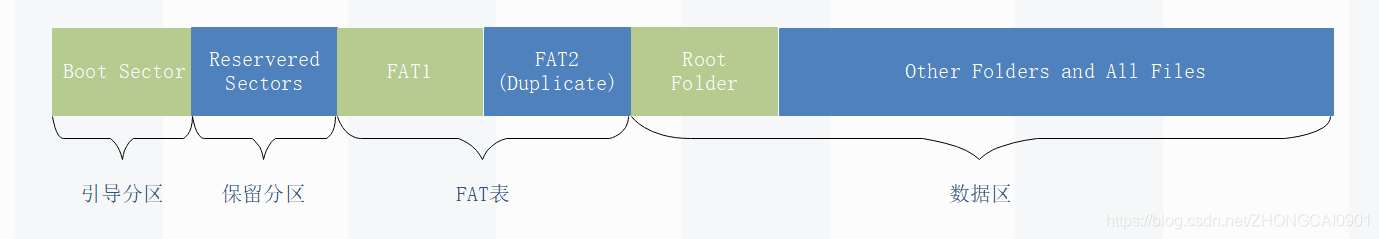
\includegraphics[width=0.9\textwidth]{FatFs.png}
			\caption{FATFS的存储结构}
		\end{figure}
	\item Boot Sector :包含BIOS参数块,该参数块存储有关卷布局和文件系统结构的信息,以及加载Windows 的引导代码。
	\item Reserved Sectors :在第一个FAT开始之前的扇区数量,包括引导扇区。 
	\item FAT 1 : 原始FAT表 。
	\item FAT 2 : FAT表的备份 。
	\item Root folder :描述根目录分区中的文件和文件夹。
	\item Other folders and all files : 包含文件系统中文件和文件夹的数据。 
	\end{itemize}
\end{itemize}

\subsubsection{ext4}
\begin{itemize}
\item 简介

第四代扩展文件系统(ext4)是Linux系统下的日志文件系统,ext4 使用 48 位的内部寻址,
理论上可以在文件系统上分配高达 16 TiB 大小的文件。在早期 ext4 的实现中有些用户空间的程序
仍然将其限制为最大大小为 16 TiB 的文件系统,但截至 2011 年,e2fsprogs 已经直接支持大于 16 TiB 大小的 ext4 文件系统。

\item 存储结构

Ext4文件系统把整个分区划分成各个block group(块组),
每个block group由superblock(超级块),block group(区块群组),
 block bitmap(区块对照表), inode bitmap(inode 对照表)和
 group descriptor以及inode table、data block组成。
	\begin{figure}[H]
		\centering
		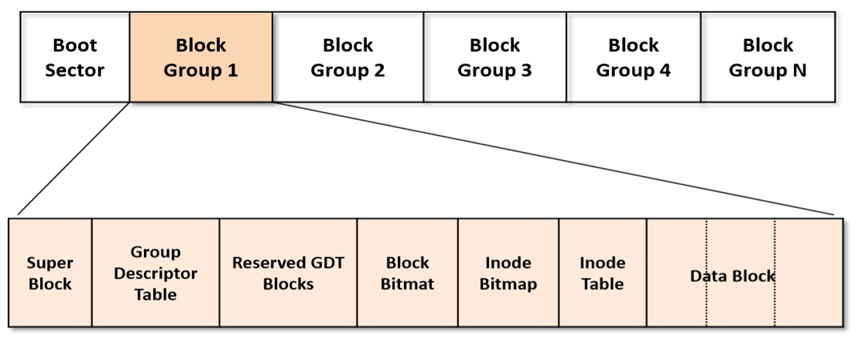
\includegraphics[width=0.9\textwidth]{ext4.png}
		\caption{ext4的存储结构}
	\end{figure}
\end{itemize}
\subsubsection{XFS}
\begin{itemize}
\item 简介
XFS是一个日志型的文件系统,能在断电以及操作系统崩溃的情况下保证数据的一致性。
XFS最早是针对IRIX操作系统开发的,后来移植到linux上,目前CentOS 7已将XFS作为默认的文件系统。
\item 存储结构
XFS文件系统内部被分为多个大小相同的“分配组(AG)”,每个AG可以看成独立维护自己空间的文件系统。

AG有如下特点:
	\begin{itemize}
	\item 一个描述整个文件系统的超级块
	\item 空闲空间管理
	\item Inode分配和追踪
	\item 反向块映射索引
	\item 数据块引用计数索引
	\end{itemize}
整个文件系统的空闲空间和所有inode数量只由第一个AG(primary)维护。通过mkfs.xfs格式化后,主AG的磁盘布局如图3所示。
	\begin{figure}[htb]
		\centering
		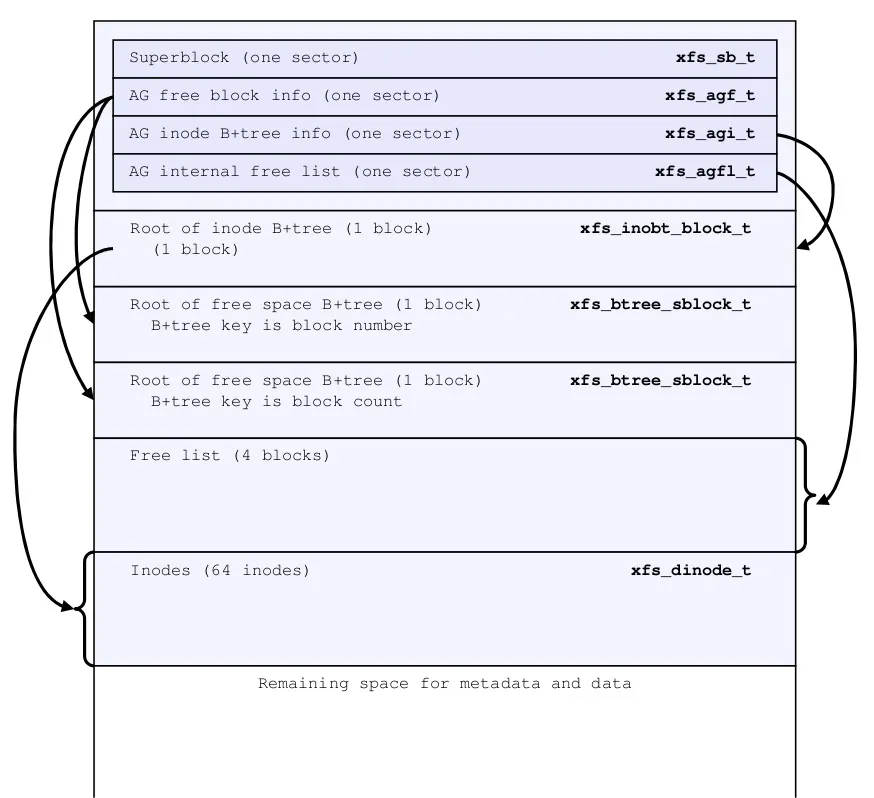
\includegraphics[width=0.9\textwidth]{XFS.png}
		\caption{XFS中AG的磁盘布局}
	\end{figure}
\end{itemize}

\subsubsection{jffs2}
\begin{itemize}
\item 简介
JFFS2(Journalling Flash File System Version2)是一个日志结构的文件系统,包含数据和原数据的节点在闪存上顺序的存储。
\item 存储结构
JFFS2在Flash上​​只有两种类型的数据实体:jffs2\_raw\_inode和jffs2\_raw\_dirent。
前者包含文件的管理信息,后者用于描述文件在文件系统中的位置。
真正的数据信息就保持在jffs2\_raw\_inode节点的后面。下图为flash中数据实体的逻辑分布,
物理上所有的数据实体离散分布,位置由写入时Flash中空闲空间位置决定。
	\begin{figure}[H]
		\centering
		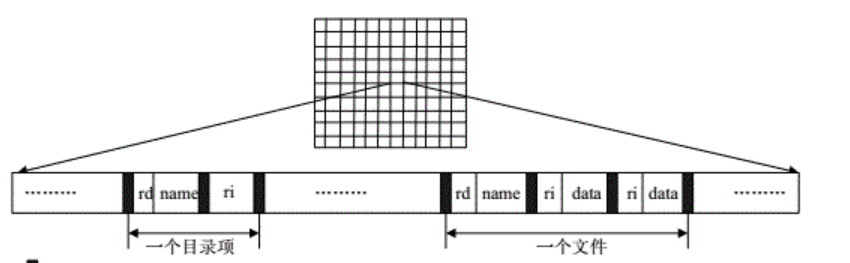
\includegraphics[width=0.9\textwidth]{jffs2.png}
		\caption{jffs2下数据实体的逻辑分布}
	\end{figure}
\end{itemize}

\subsubsection{ubifs}
\begin{itemize}
\item 简介
UBIFS(),用于裸的flash设备,作为jffs2的后继文件系统之一。
\item 存储结构
ubifs文件系统将整个磁盘空间划分为superblock、master、log、lpt、orphan和main六个区域,其区域划分如下所图所示:

	\begin{figure}[H]
		\centering
		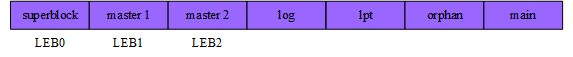
\includegraphics[width=0.9\textwidth]{UBIFS.png}
		\caption{ubifs对磁盘空间的划分}
	\end{figure}
	\begin{itemize}
		\item superblock区域固定占用LEB0,master区域固定占用LEB1和LEB2,其他区域占据的LEB数量则视该文件系统分区实际占有的总的LEB数量而定,orphan区域一般占用1到2个LEB。superblock区域保存文件系统的固定参数,参数在格式化时写入,除了leb\_cnt元素和UBIFS\_FLG\_SPACE\_FIXUP标志位会在首次挂载时被改变,其他元素皆为只读。
		\item master区域中的两个LEB相互备份,以确保在异常掉电的情况能够恢复master区域的内容。master区域的数据在每次发生commit的时候进行更新。
		\item log区域记录日志数据的存储位置lnum:offs。ubifs是一种日志文件系统,文件数据采用异地更新的方式(out\_of\_place\_update),即文件数据的更新不会每次都同步到flash,而是记录到日志区,当日志区的数据累计到一定程度时,才将数据同步到flash中。
		\item lpt区域记录了磁盘空间中各个LEB的状态(free、dirty、flag),用于实现对LEB的分配、回收和状态查询。
		\item main区域则保存文件的数据和索引。
	\end{itemize}
\end{itemize}

\subsubsection{f2fs}
\begin{itemize}
\item 简介
F2FS(Flash-Friendly File System)是一种闪存文件系统,此文件系统起初是为了NAND闪存的存储设备设计(诸如固态硬盘、eMMC和SD卡),这些设备广泛存在于自移动设备至服务器领域。
\item 存储结构
F2FS将整个卷分成多个段(segment),每个段固定为2 MB。一个节(section)由连续的段组成,一个区(zone)由一组节组成。默认情况下,节与区被设置为相同的大小,但用户可以用mkfs轻松修改大小。F2FS将整个卷划分为六个区域,除了超级块(superblock)以外的所有区都由多个段组成。

	\begin{itemize}
		\item 超级块(Superblock)
		超级块位于分区起始处,共有两个副本以避免文件系统损坏。它包含基本的分区信息和一些默认的F2FS参数。
		\item 检查点(Checkpoint)
		检查点包含文件系统信息,有效NAT/SIT集的位图,孤立inode列表,以及当前活动段的摘要条目。
		\item 段信息表(SIT)
		段信息表包含主区域块的有效块数量和有效位图。
		\item 节点地址表(NAT)
		节点信息表主区域节点块的地址表。
		\item 段摘要区(SSA)
		段摘要区包含的条目包含主区域数据和节点块的所有者信息。
		\item 主区域(Main Area)
		主区域包含文件和目录数据及其索引。
	\end{itemize}
\end{itemize}

\subsubsection{romfs}
传统型的Romfs文件系统是最常使用的一种文件系统,它是一种简单的、紧凑的、只读的文件系统,不支持动态擦写保存;它按顺序存放所有的文件数据,因此在系统运行时,可以获得可观的RAM节省空间
romfs的主要目的是拥有一个非常小的内核,它只链接了这个文件系统,然后可以在以后使用当前的模块实用程序加载任何模块。

romfs在块设备上运行,并且底层结构非常简单。为了快速访问,每个可访问的结构都从16字节边界开始。文件占用的最小空间为32字节。
romfs系统中最大文件的大小理论上可以达到4G,文件名的大小一般小于16字节,而且整个文件系统都是以16字节来对齐。romfs映像开始16字节对应struct\ romfs\_super\_block结构体,后为romfs映像的卷标。
紧随卷标之后的就是第一个文件的文件头romfs\_inode结构,共16字节,之后就是文件名,也是16字节对齐,然后才是文件内容。其中在每个文件的文件头中的前4字节(不包括低4位)为下一个文件头在romfs映像中的偏移。
下图左侧为superblock的结构,右为romfs\_inode即文件头的格式。
	\begin{figure}[H]
		\centering
		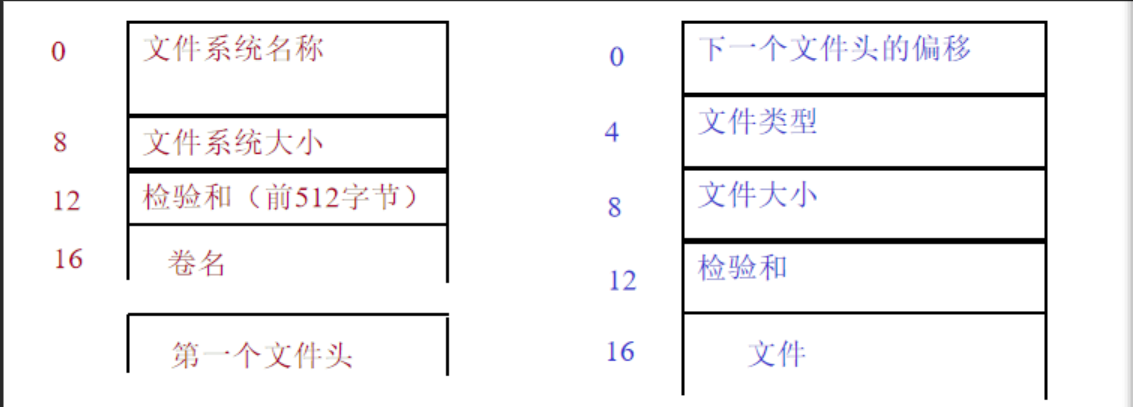
\includegraphics[width=0.9\textwidth]{romfs.png}
		\caption{romfs的文件系统布局和文件结构}
	\end{figure}
\subsubsection{小结}
根据以上对文件系统的调研和小组讨论,我们初步决定基于FreeRTOS-Plus-FAT添加jffs2和romfs作为可支持的文件系统。其他则作为参考和备选方案。

\subsection{虚拟文件系统 - Linux}
\subsubsection{概述}

虚拟文件系统(VFS)是操作系统中的一个抽象层,它允许不同的文件系统(例如
\href{https://en.wikipedia.org/wiki/Ext4}{ext4}、
\href{https://en.wikipedia.org/wiki/NTFS}{NTFS}
和
\href{https://en.wikipedia.org/wiki/File_Allocation_Table}{FAT32})
以一致的方式呈现其内容。虚拟文件系统为应用程序提供了一个通用的文件系统
API
接口,
亦可以用于透明地访问本地与网络存储设备而不让客户端应用程序察觉到差别。
它可以用来弥合
Windows, macOS,以及 Unix
的文件系统之间的差异,以便于应用程序访问这些不同类型的本地文件系统上的文件,
而无需得知其正在访问的文件系统类型。

虚拟文件系统规定了操作系统内核与具体文件系统之间的接口(或合同),
因此,只需满足这些借口所需的条件即可向内核添加对新文件系统的支持。
但是,这些文件接口所需要满足的条件可能随着操作系统版本的更新而发生变化,
这便会要求对某一具体文件系统的支持程序进行一定的修改,
并且重新编译操作系统内核。当然,操作系统的开发者也可以选择向后兼容的更新改版,
使之前版本的具体文件系统支持程序继续工作在更新后的操作系统上。

\begin{figure}[H]
    \centering
    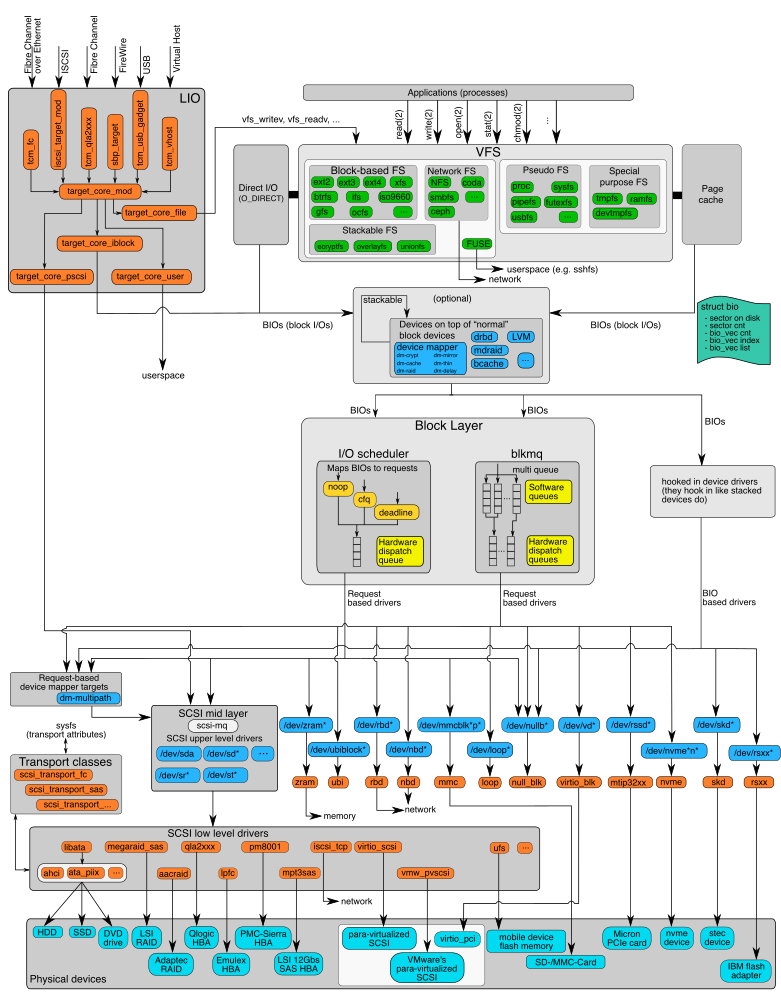
\includegraphics[width=0.6\textwidth]{The_Linux_Storage_Stack_Diagram.png}
    \caption{The Linux Storage Stack Diagram}
\end{figure}

上图为 VFS 层在 Linux 内核存储栈中相对各个部分的位置。

Linux文件系统的灵活性和可扩展性是抽象接口集的直接结果。
这个接口集的核心是便虚拟文件系统开关(VFS)。

VFS为上层应用程序提供一组标准接口,
以便在多种文件系统上执行文件读写,
并支持在一个或多个底层设备上同时使用多个文件系统。
此外,这些文件系统并不需要是静态的,它们可能会随着存储设备的瞬态性而改变。
例如,一个典型的
Linux 桌面系统支持可用硬盘上的 ext3 文件系统,以及可用
\href{https://en.wikipedia.org/wiki/CD-ROM}{CD-ROM} 上的
\href{https://en.wikipedia.org/wiki/ISO_9660}{ISO 9660} 
文件系统(也称为
CD-ROM 文件系统或 CDFS)。
随着 CD-ROM 的插入和移除,Linux
内核必须适应这些具有不同内容和结构的新文件系统。
远程文件系统可以通过网络文件系统(NFS)访问。同时,Linux
可以从本地硬盘上的 Windows/Linux 双启动系统中挂载 NT
文件系统(NTFS)分区,并从中读取和写入数据。

同样,可移动的 USB
闪存驱动器(UFD)可以热插拔,提供另一个文件系统。
在此期间,这些相同的文件接口,允许将底层文件系统和物理设备抽象出来,
以便用户使用,见下图。

\begin{figure}[H]
    \centering
    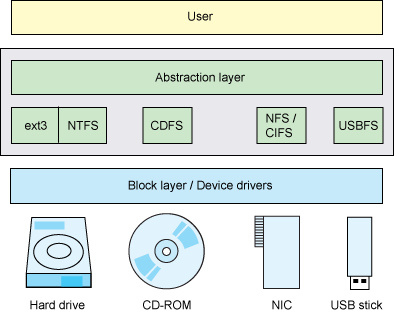
\includegraphics[width=0.4\textwidth]{figure1.jpg}
    \caption{文件系统和物理设备}
\end{figure}

\subsubsection{Layer Abstraction}

\begin{figure}[H]
    \centering
    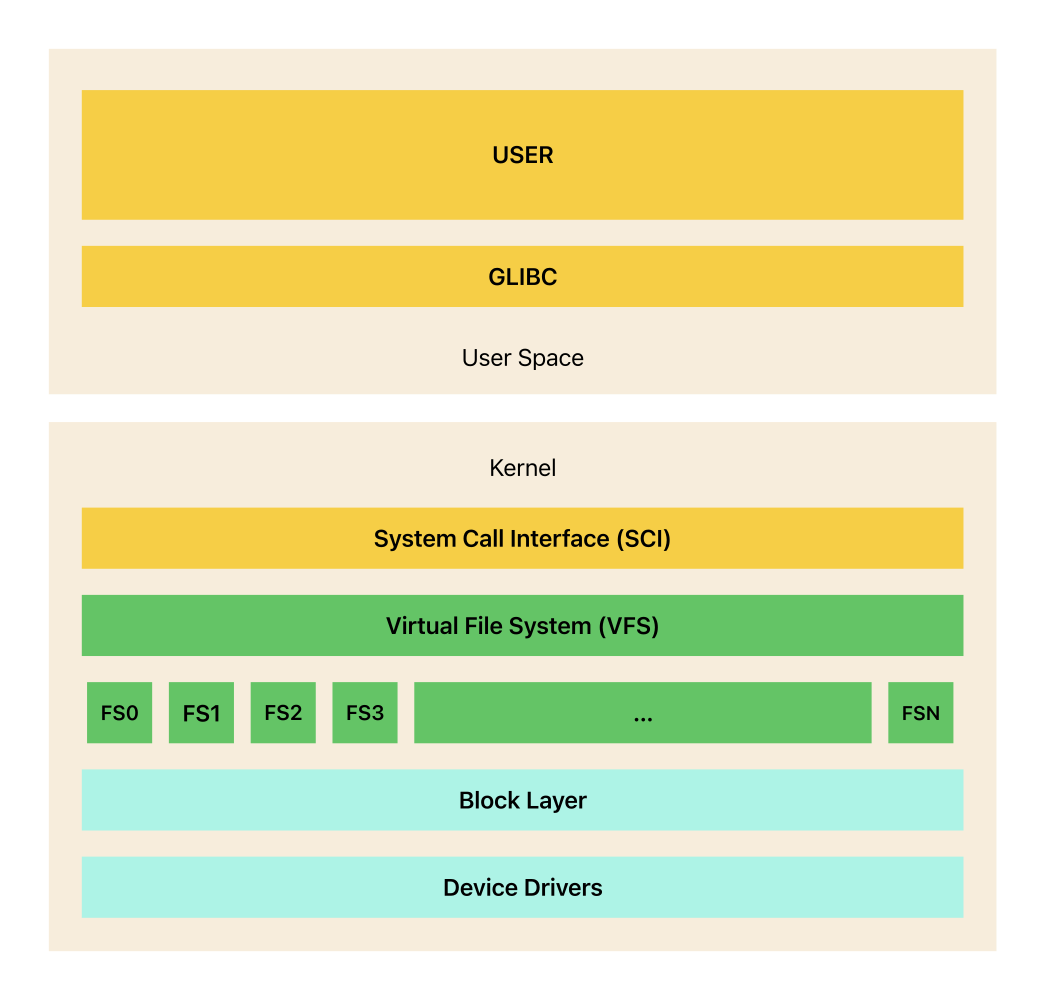
\includegraphics[width=0.6\textwidth]{The layered architecture of the VFS.png}
    \caption{The layered architecture of the VFS}
\end{figure}

接下来,对 Linux VFS 提供的抽象特性添加一些具体的架构。上图展示了从 VFS
的角度看 Linux 栈的高层视图。在 VFS
的上方是标准内核系统调用接口
(\href{https://en.wikipedia.org/wiki/Scalable_Coherent_Interface}{SCI})。
这个接口允许用户空间的调用从不同的地址空间过渡到内核中。
在这个域中,一个用户空间应用程序激发
\href{https://en.wikipedia.org/wiki/POSIX}{POSIX} open call 通过
\href{https://en.wikipedia.org/wiki/GNU}{GNU} C
库(\href{https://en.wikipedia.org/wiki/Glibc}{glibc})v
进入内核并进入系统调用解多路器。最终,使用
\code{sys\_open} 调用 VFS。

VFS 提供抽象层,
将 POSIX API
与特定文件系统实现该行为的细节分离。
关键在于,
无论底层文件系统是
ext3还是Btrfs,
打开,
读取,
写入或关闭的 API
系统调用都是相同的。
VFS提供了一个底层文件系统可以继承的共同文件模型
(它们必须能够实现各种
POSIX API
的函数)。
在VFS之外,
还有一个抽象层将底层物理设备隐藏起来,
这些底层物理设备可以是是磁盘、
磁盘分区、
网络存储实体、
内存或任何能够存储信息,
甚至是短暂存储介质。

除了将底层文件操作与可用文件系统联系起来,
VFS还将底层块设备与可用文件系统联系起来。

\subsubsection{Superblock}

Superblock 是一个关于文件系统高级元数据的容器。
Superblock
是一个存在于磁盘(实际上是多个位置上的冗余信息)
和内存中的结构。它是处理磁盘上文件系统的基础,
因为它定义了文件系统的管理参数,例如,总块数、可用块数、根索引节点。

在磁盘上,superblock
向内核提供有关磁盘上文件系统结构的信息。
在内存中,superblock
提供了管理已挂载文件系统所需的信息和状态。因为 Linux
支持在同一时间挂载多个并发文件系统,所以每个 \texttt{super\_block}
结构都在一个 \texttt{super\_blocks} 列表中维护(\texttt{super\_blocks}
在 \texttt{./linux/fs/super.c} 中定义,\texttt{super\_block}结构在
\texttt{/linux/include/fs/fs.h} 中定义)。

\begin{figure}[H]
    \centering
    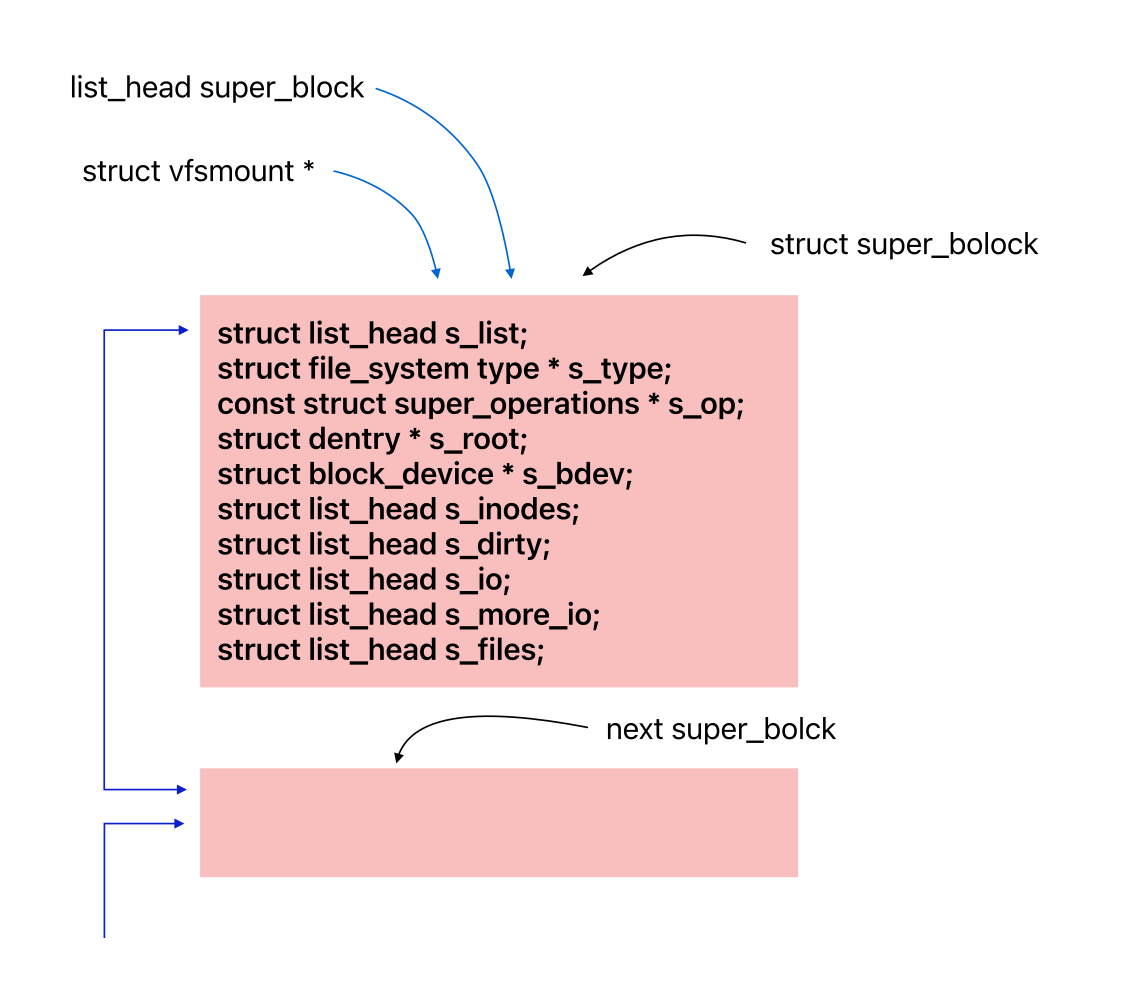
\includegraphics[width=0.6\textwidth]{Simplified view of the super_block structure and its related elements.png}
    \caption{Simplified view of the super\_block structure and its related elements}
\end{figure}

上图为 superblock 及其元素的简化视图。\texttt{super\_block}
结构引用了许多封装其他信息的结构体。例如,\texttt{file\_system\_type}
结构体维护文件系统的名称(如ext3)以及获取和删除 \texttt{super\_block}
的各种锁和函数。\texttt{file\_system\_type}
对象通过著名的\texttt{register\_file\ system} 和
\texttt{unregister\_file\ system} 函数进行管理(见
\texttt{./linux/fs/file\ systems.c})。\texttt{super\_operations}
结构定义了读写索引节点以及更高级别操作的多个函数,如重新挂载。
根目录条目(dentry)对象与此文件系统所在的块设备同样在此被缓存。最后,superblock
提供多个列表来管理索引节点,包括
\texttt{s\_inodes}(所有索引节点的列表)、
\texttt{s\_dirty}
(所有脏索引节点的列表)、\texttt{s\_io}
和
\texttt{s\_more\_io}(停止进行写回)、
\texttt{s\_files}(给定文件系统的所有打开文件的列表)。

另外,Linux 内核中还有另一个管理对象称为
\texttt{vfsmount},它提供有关挂载的文件系统的信息。这些对象的列表引用了
superblock 并定义了挂载点,文件系统所在的 \texttt{/dev}
设备的名称,以及其他更高级别的附加信息。


\subsubsection{The Index Node (inode)}
Linux 通过一个称为
inode(索引节点)的对象来管理文件系统中的所有对象。一个 inode
可以指向一个文件、一个目录或另一个对象的符号链接。因为文件用于表示其他类型的对象比如设备或内存,inode
也用于表示它们。

请注意,这里提到的 inode 是 VFS 层的 inode(内存
inode)。事实上,每个文件系统还包括一个
inode,它位于磁盘上,能够提供有关特定文件系统对象的详细信息。

VFS inode 使用
slab分配器(来自 \texttt{inode\_cache})进行分配。其由描述 inode
与内容以及可能在 inode 上执行的各种操作的数据和操作组成。

\begin{lstlisting}[language=C]
struct list_head i_dentry;
struct timespec i_atime;
struct timespec i_mtime;
struct timespec i_ctime;
gid_t i_gid;
uid_t i_uid;
loff_t i_size;
const struct file_operations * i_fop;
const struct inode_operations * i_op;
struct address_space * i_maping;
struct address_space * i_data;
…
\end{lstlisting}

以上是一个简单的 VFS inode 示例,包含多个列表,其中一个列表引用了指向此
inode 的
dentries。对象级元数据包括熟悉的操作时间(创建时间、访问时间、修改时间),以及所有者和权限数据(group-id、user-ID
和 permissions)。inode
引用了可能在其上执行的文件操作,其中大多数直接映射到系统调用接口(例如,\texttt{open}、\texttt{read}、\texttt{write}
和 \texttt{flush})。还有一个引用 inode 特定操作的结构(如
\texttt{create}、\texttt{lookup}、\texttt{link}、\texttt{mkdir}
等)。最后,还有一个结构来管理由地址空间对象表示的对象的实际数据。\texttt{address\ space}
对象是一个管理 inode
在页面缓存中的各个页面的对象。地址空间对象用于管理文件的页面,并将文件段映射到各个进程地址空间中。地址空间对象配有自己的操作集(\texttt{writepage}、\texttt{readpage}、\texttt{releasepage}
等)。

\subsubsection{Directory Entry (dentry)}

Linux 中的另一个对象,称为 \texttt{dentry}
对象,它用于管理文件系统的分层结构。文件系统有一个根 dentry(在
\texttt{super\_block} 中被引用),这是唯一一个没有 parent 的
dentry。所有其他 dentry 都有 parent,有些有 children。例如,如果打开了由
\texttt{/home/user/name} 组成的文件,则将会有四个 dentry
对象被创建:一个用于根目录 \texttt{/},一个用于根目录的 \texttt{home}
条目,一个用于 \texttt{user} 目录的 \texttt{name} 条目,最后,一个用于
\texttt{user} 目录的 \texttt{name} 条目的
\texttt{dentry}。通过这种方式,dentry
在今天使用的分层文件系统中拥有非常清晰的映射。

dentry 对象由 \texttt{dentry} 结构(位于
\texttt{./linux/include/fs/dcache.h})定义。
它包括一些用于跟踪该条目与文件系统中其他条目关系,
以及物理数据(例如文件名)的元素。

\begin{lstlisting}[language=C]
struct wuper_block * d_sb;
struct dentry * d_parent;
struct list_head d_subdirs;
struct dentry_operations * d_op;
unsigned char d_iname[];
struct inod * d_inode;
…
\end{lstlisting}

以上展示了 dentry 对象的简化视图。dentry 引用了 super\_block,而
\texttt{super\_block}
定义了包含该对象的特定文件系统实例。接下来是该对象的 parent
dentry(父目录),后跟包含在列表中的 child
dentry(如果该对象恰好是目录),然后定义了 dentry 的操作(包括
\texttt{hash},\texttt{compare},\texttt{delete},\texttt{release}
等操作)。对象的名称随后被定义,该名称在 dentry 中而不是 inode
本身中保存。最后,提供了对VFS inode的引用。

请注意,dentry
对象仅存在于文件系统内存中,不会存储在磁盘上。只有文件系统 inode
被永久存储,而 dentry
对象用于提高性能。可以在\texttt{./linux/include/dcache.h} 中查看 dentry

\subsubsection*{File Object}

对于 Linux
系统中每个打开的文件,都存在一个文件对象。
该对象包含给定用户的打开实例的相关信息。
文件对象的一个较为简化的视图下面中提供。

\begin{lstlisting}[language=C]
struct path    f_path;
struct dentry (f_path, dentry);
const struct file_operations * f_op;
unsigned int f_flags;
fmode_t f_mode;
lodd_t f_ops;
…
\end{lstlisting}

如图所示,路径结构提供了对 dentry 和 vfsmount
的引用。为每个文件定义了一组文件操作,
这些操作是众所周知的文件操作(例如打开、关闭、读取、写入、刷新等)。
还定义了一组标志和权限(包括组和所有者)。
最后,为特定的文件实例定义了有状态数据,
例如文件的当前偏移量。
\subsubsection{小结}
VFS(虚拟文件系统)
是 Linux
内核中的一个抽象层,它提供了一组标准的文件系统操作,这些操作可以在不同的文件系统上实现。
VFS
的内部架构由一个提供文件系统抽象的分派层和一些缓存组,
以此能够提高文件系统操作的性能。

\begin{figure}[H]
    \centering
    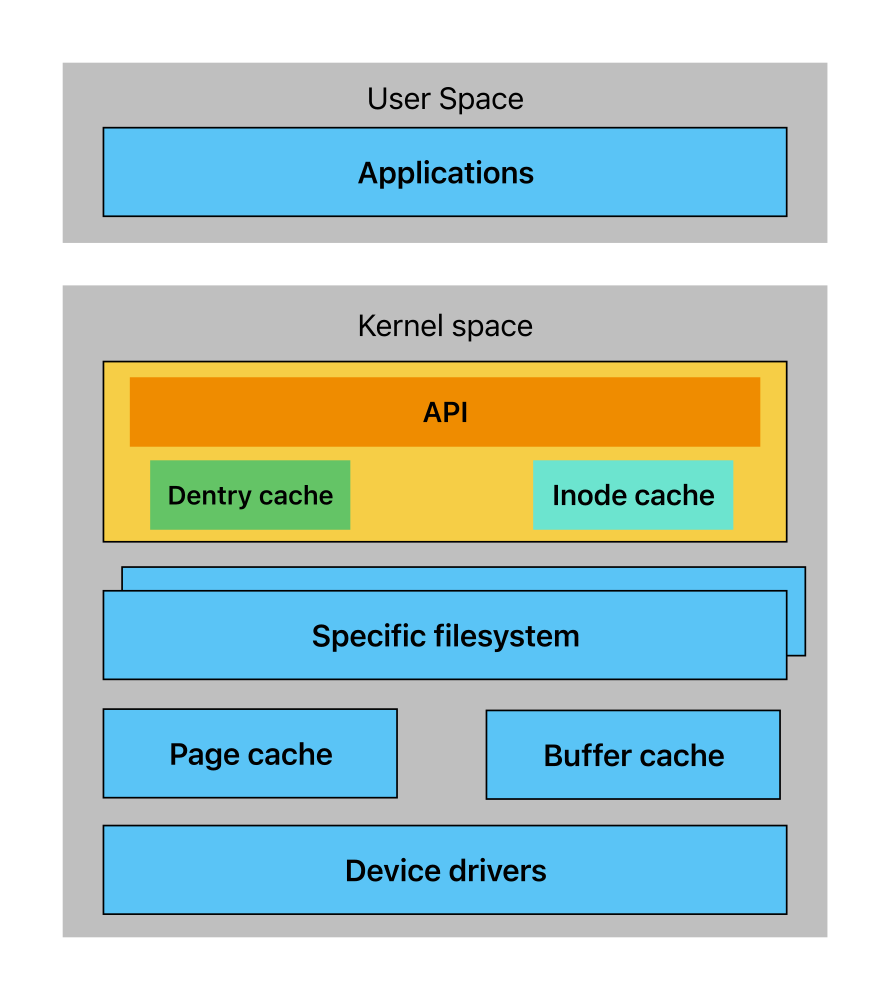
\includegraphics[width=0.6\textwidth]{High-level view of the VFS layer.png}
    \caption{VFS 层的高级视图}
\end{figure}

在 VFS 中,两个主要的动态管理对象包括 \texttt{dentry} 和 \texttt{inode}
对象。将这些对象缓存可以提高对底层文件系统的访问性能。当打开一个文件时,\texttt{dentry}
缓存将被填充以表示路径所代表的目录级别的条目。同时还会创建一个 inode
表示文件的对象。\texttt{dentry}
缓存使用哈希表构建,由对象名称进行哈希。\texttt{dentry} 缓存的条目是从
\texttt{dentry\_cache} 的 slab
分配器中分配的,并使用最近最少使用(\href{https://en.wikipedia.org/wiki/Cache_replacement_policies\#LRU}{LRU})
算法来修剪条目以应对内存压力。与
\texttt{dentry} 缓存相关的函数可以在 \texttt{./linux/fs/dcache.c}和
\texttt{./linux/include/linux/dcache.h} 中找到。

\texttt{inode}
缓存是由两个列表和一个哈希表实现的,这样可以实现更快地查找。第一个列表定义了当前正在使用的
\texttt{inodes},第二个列表定义了未使用的 \texttt{inodes}。正在使用的
\texttt{inodes} 也存储在哈希表中。从 \texttt{inode\_cache} 的 slab
分配器中分配单个 \texttt{inode} 缓存对象。与 \texttt{inode}
缓存相关的函数可以在\texttt{./linux/fs/inode.c} 与
\texttt{./linux/include/fs.h} 中找到。

从实现来看,\texttt{dentry} 缓存是 \texttt{inode} 缓存的主控制器。当
\texttt{dentry} 对象存在时,\texttt{inode} 对象也会存在于 \texttt{inode}
缓存中。在 \texttt{dentry} 缓存上执行查找,将导致在 \texttt{inode}
缓存中获得一个对象。

\subsection{虚拟文件系统 - 嵌入式}
\subsubsection{概述}
本部分主要介绍了 \texttt{FreeRTOS-Plus-FAT} 以及 \texttt{RT-Thread} 
中的文件系统实现细节。

在早期的嵌入式系统中,需要存储的数据比较少,
数据类型也比较单一,往往使用直接在存储设备中的指定地址写入数据的方法来存储数据。
然而随着嵌入式设备功能的发展,需要存储的数据越来越多,也越来越复杂,
这时仍使用旧方法来存储并管理数据就变得非常繁琐困难。
因此需要新的数据管理方式来简化存储数据的组织形式,需要新的文件系统设计。

\subsubsection{\texttt{FreeRTOS-Plus—FAT}}
通过阅读源代码,可以简单分类此项目的文件组织如下。
\begin{itemize}
\item 主要
\begin{itemize}
    \item \texttt{ff\_dir}: 用于访问文件夹中内容
    \item \texttt{ff\_fat}: 用于访问 \texttt{FAT} 文件系统
    \item \texttt{ff\_file}: 用于文件读写
    \item \texttt{ff\_ioman}: 管理缓存和挂载读写对象(介质)
    \item \texttt{ff\_format}: 格式化或分区介质
    \item \texttt{ff\_locking}: 加锁?
    \item \texttt{ff\_memory}: 从内存读取数据
    \item \texttt{ff\_stdio}: 用于文件管理(统计),相对路径转换
    \item \texttt{ff\_sys}: 用于映射文件系统到根目录
\end{itemize}
\item 辅助
\begin{itemize}
    \item \texttt{ff\_headers}: 管理所有头文件
    \item \texttt{ff\_time}: 获取时间
    \item \texttt{ff\_error}:  用于错误处理
    \item \texttt{ff\_crc}: 用于计算 \texttt{CRC}(循环检验码)
    \item \texttt{ff\_string}: 字符串库
\end{itemize}
\item 驱动
\begin{itemize}
    \item 各处理器相应的文件系统驱动
\end{itemize}
\end{itemize}

\paragraph{\texttt{ERRNO} 值} \texttt{FreeRTOS-Plus-FAT} 文件系统的标准 API 与标准 C 库使用相同的 \texttt{errno} 值。
标准 C 库中的文件相关函数返回 0 表示通过,返回 -1 则表示失败。如果返回 -1,则失败的原因 存储在名为 \texttt{errno} 的变量中,须单独检查。 
同样,\texttt{FreeRTOS-Plus-FAT} 的标准 API 返回 0 表示通过,返回 -1 则表示失败, 该 \texttt{API} 还会针对各项 \texttt{RTOS} 任务维护 \texttt{errno} 变量。

\subsubsection{\texttt{RT-Thread}}
此文件系统有较多简介,可供设计参考,它的特点是:
\begin{itemize}
    \item 为应用程序提供统一的 \texttt{POSIX} 文件和目录操作接口:\texttt{read}、\texttt{write}、\texttt{poll/select} 等。
    \item 支持多种类型的文件系统,如 \texttt{FatFS}、\texttt{RomFS}、\texttt{DevFS} 等,并提供普通文件、设备文件、网络文件描述符的管理。
    \item 支持多种类型的存储设备,如 \texttt{SD Card}、\texttt{SPI Flash}、\texttt{Nand Flash} 等。
\end{itemize}
\paragraph{POSIX 文件系统接口}

\texttt{POSIX} 表示可移植操作系统接口,\texttt{POSIX} 标准定义了操作系统应该为应用程序提供的接口标准,是 \texttt{IEEE} 为要在各种 \texttt{UNIX} 操作系统上运行的软件而定义的一系列 \texttt{API} 标准的总称。

此标准意在期望获得源代码级别的软件可移植性。换句话说,为一个 \texttt{POSIX} 兼容的操作系统编写的程序,应该可以在任何其它 \texttt{POSIX} 操作系统(即使是来自另一个厂商)上编译执行。\texttt{RT-Thread} 支持 \texttt{POSIX} 标准接口,因此可以很方便的将 Linux/Unix 的程序移植到 RT-Thread 操作系统上。

\paragraph{虚拟文件系统层}
用户可以将具体的文件系统注册到 \texttt{DFS} 中,如 \texttt{FatFS}、\texttt{RomFS}、\texttt{DevFS} 等,具体介绍请参考其他小节。

\paragraph{设备抽象层}
设备抽象层将物理设备如 \texttt{SD Card}、\texttt{SPI Flash}、\texttt{Nand Flash},抽象成符合文件系统能够访问的设备,例如 \texttt{FAT} 文件系统要求存储设备必须是块设备类型。

不同文件系统类型是独立于存储设备驱动而实现的,因此把底层存储设备的驱动接口和文件系统对接起来之后,才可以正确地使用文件系统功能。
\subsubsection{小结}
设计 \texttt{VFS} 时,可以参考 \texttt{RT-Thread} 的三层结构组织形式、\texttt{FreeRTOS-Plus-FAT} 的API函数设计理念,将 \texttt{FreeRTOS-Plus-FAT} 继续拓展优化。

例如,可通过以下几点提高\textbf{兼容性}。(利用 \texttt{POSIX} 文件系统接口和与 \texttt{FreeRTOS-Plus-POSIX} 的结合将有可能方便地运行从 \texttt{Linux/Unix} 上移植的程序。
虽然目前 \texttt{FreeRTOS-Plus-POSIX} 对 \texttt{POSIX API} 的支持还不够充分,但是随着开发实用价值将逐渐上升。)

\begin{itemize}
    \item 继续采用标准 \texttt{eerno} 值
    \item 添加 \texttt{POSIX} 文件系统接口
    \item 添加支持的文件系统(磁盘文件系统、闪存文件系统)
    \item 拓展支持的实用函数
\end{itemize}

\subsection{文件系统开发}
	\subsubsection{概述}
	一个文件系统的开发需要考虑多方面的要素,比如:文件系统的类型、大小、性能要求等。如果在嵌入式设备上开发更需要考虑设备的存储容量和处理器速度等因素。大体来说,评价一个文件系统可以参考以下指标:
	
	1. 可靠性:长时间运行中不出现数据损坏或丢失
	
	2. 安全性:保护用户数据不被恶意软件或黑客攻击
	
	3. 可扩展性:可以支持更大的存储量和更多的文件
	
	4. 兼容性:可以在不同的操作系统和设备上使用
	
	5. 性能:文件系统的读写速度与响应时间
	
	以下对可靠性、安全性、性能相关内容做了较为详细的阐述并对本项目的开发语言选择及效果评测提出建议。
	\subsubsection{可靠性}
	提升文件系统的可靠性的方法主要是两种:避错和容错。其中,避错是指尽量避免出现错误,而容错则是指在出现错误时,能够自动或者半自动地恢复系统。在实际操作中,大多考虑通断电时候文件系统是否仍然可靠。高可靠文件系统的设计原理本质上是copy-on-write,设置transaction point,保证transaction point提交的时候,所有依赖的数据都被正确的写入即可,\textbf{所以,可靠性的提升实际上是利用硬件空间,且在RTOS上是难以与实时性共存的。}
	\begin{quote}
		\zihao{-6}\songti
		COW(copy-on-write 的简称),是一种计算机设计领域的优化策略,其核心思想是:如果有多个调用者(callers)同时要求相同资源(如内存或磁盘上的数据存储),他们会共同获取相同的指针指向相同的资源,直到某个调用者试图修改资源的内容时,系统才会真正复制一份专用副本(private copy)给该调用者,而其他调用者所见到的最初的资源仍然保持不变。这过程对其他的调用者都是透明的(transparently)。此作法主要的优点是如果调用者没有修改该资源,就不会有副本(private copy)被创建,因此多个调用者只是读取操作时可以共享同一份资源
		
		transaction point是文件系统处于一致状态的时间点。它用于确保数据的完整性和可靠性。设置事务点后,将记录在该点之后对文件系统所做的所有更改。如果文件系统出现问题,可以将其还原到事务点时的状态。这可确保数据不会丢失,并且文件系统保持可靠。
	\end{quote}
	
	\subsubsection{安全性}
	提升文件系统的安全性需要注意以下几个方面:
	
	开发语言:开发语言在一定程度上影响了文件系统的安全性,这是由语言自身特性决定的。
	
	加密算法:为追求文件系统的安全性也可使用加密算法进行加密。
	
	\textbf{值得提出的问题是,}本项目注重于VFS的开发,那么单纯的VFS安全性提升对整个文件系统以及操作系统的安全性提升应当是有限的,无论是改用更加安全的开发语言抑或是使用加密算法都应该更需要部署在文件系统和操作系统上。
	\subsubsection{性能}
	性能是衡量文件系统读写数据、处理并发请求以及应对不同工作负载的速度和效率的参数,可以说是文件系统优劣的最直观体现。以下是一些进行文件系统性能测试的工具:
	
	1.Filebench:一个可以生成各种合成工作负载的工具,可以模拟真实的应用服务器场景,比如web服务器、邮件服务器、数据库服务器等,可以使用Filebench测试不同文件系统在不同工作负载下的性能,并比较结果 .
	
	2.FIO:一个可以使用可配置的工作负载生成器运行各种 I/O 测试的工具。可以使用 FIO 来测试使用不同 I/O 模式、块大小、队列深度等的不同文件系统的性能。
	
	3.IOzone:一个可以使用读、写、重读、重写、随机读/写等各种操作来测试文件系统性能的工具。可以使用IOzone来测试不同文件系统的性能使用不同的文件大小、记录长度、线程数等。
	
	RTOS的文件系统的实时性要求较高,在完成VFS应使用以上工具或其它工具测试整个文件系统的效率与性能。
	
	\subsubsection{开发语言的选择}
	\textcolor{red}{本地文件系统或虚拟文件系统的编程语言不必与操作系统相匹配,实际上文件系统只需与VFS的接口进行交互,而虚拟文件系统是物理文件系统实现的抽象,故而仅需注意不同编程语言间的API接口即可}。
	
	\textbf{RTOS的安全问题}
	
	RTOS 受到其运行的硬件平台的限制,若对缺少存储器保护的硬件加以保护,其安全级别会受到限制。但存储器和虚拟机可以更高水平的安全性支持引导。诸如 SE Linux、 Green Hills Integrity 和LynuxWorks LynxSecure Embedded Hypervisor 以及 LynxOS-SE RTOS 内的安全策略可比典型 RTOS 提供可靠得多的保护,同时也带来了高成本的问题,所以开发者需进行权衡。
	
	\textbf{RTOS的性能问题}
	
	RTOS最鲜明的特征是实时性,换而言之,是其管理资源 (包括时间和存储器) 的能力。
	
	时序问题与中断响应时间有关,但资源管理时序问题也会同时出现。中断能解决了一系列时序问题,但各应用仍必须利用资源。
	 
	考虑存储器分配情况。许多实时应用不采用动态存储器分配,以确保存储器分配和回收时所产生的不同不会变成一个问题。需要动态存储器分配的应用常把存储器划分为实时和非实时。后者处理动态存储器分配。典型情况下,在使用前,实时部分必须被分 配有足够的存储器。
	
	\textbf{语言对比}
	
	以下对C/C++和Rust的优劣作了对比:
	
	1. C/C++
	\textbf{C/C++的使用有利于实时性的提升},原因在于其存储器和其它资源的用法显式的,且更接近底层,能直接操作硬件。
	\textbf{但同时,在C/C++开发出来的年代,安全性问题并未得到和性能问题一样的重视导致其很容易出现漏洞},包括但不限于以下
	
	1.   \textbf{释放后使用/双重释放错误}:由于需要手动管理内存,导致需要在`free`时小心翼翼
	
	2. \textbf{悬空指针}:可能导致空指针引用等不安全行为
	
	3.  \textbf{缓冲区溢出错误}:这是造成大量漏洞和导致被攻击的原因
	
	4.  \textbf{数据竞争}:数据的不安全并发修改
	
	5.  \textbf{未初始化的变量}:会引发一系列未定义行为
	
	这也导致了在编写、调试程序时通常需要花费大量的时间来解决内存或数据竞争问题,而人肉 code review 大大降低了效率,也给后续的维护造成了极大的挑战。
	
	\textbf{Rust}
	
	\textbf{Rust对实时性的支持是不如C/C++的},但是其速度仅仅\href{https://blog.famzah.net/2016/09/10/cpp-vs-python-vs-php-vs-java-vs-others-performance-benchmark-2016-q3/}{比C++慢7\%}
	
	\textbf{安全性上,Rust 针对内存安全做了严格的限制。}安全地读写内存 
	
	1.在限定时间和空间范围内读写内存
	
	2. 防止被他人意外修改或释放
	
	3. 避免访问空指针和野指针 安全地释放内存
	
	4. 在恰当的时机释放
	
	5. 确保释放,不遗漏
	
	6. 仅释放一次 
	
	总体来说 它不允许空指针、悬空指针或数据竞争。其丰富的类型系统和所有权模型保证了内存安全和线程安全,使得能够在编译时消除许多类别的错误。也就是说,一段能跑起来的代码大概率是安全的。
	\subsubsection{小结}
	1. 开发语言的选择不存在理论上的最优选择,但是建议在C、Rust中选择一个。值得指出的是,如果仅仅是VFS采用Rust语言,文件系统的安全性是否能得到较大提升,就目前的知识而言,文件系统的安全性主要还是由其本身决定的。
	
	2. 开发完VFS后,FreeRTOS的性能等参数仍有待测试。

\section{立项依据}
如前所述,嵌入式系统FreeRTOS迫切需要一个完整功能的文件系统来提供对大容量存储空间的高效管理。目前已有的不少嵌入式系统的文件系统架构及API设计都值得我们学习,例如通过支持POSIX文件接口来提高可移植性及兼容性、通过支持更多的实用函数来提高用户编写程序的效率等。
FreeRTOS原有的文件系统模块目前仅支持FATFS,且功能和设计都比较简单,适合进行多种拓展来形成一个全面的虚拟文件系统。同时,在大多数嵌入式系统的文件系统文档中仅介绍了基础架构,并未提及性能及安全优化两点,我们认为可以在此两点处对原有的基础文件系统进一步提升。
总的来说,我们的项目希望具有如下关键特性:
\begin{itemize}
	\item 多种文件系统支持
	\item 兼容 POSIX 文件接口
	\item 支持加密存储
	\item 文件权限管理
	\item 高效备份
	\item 多方面性能优化
	\item MMU(远期)
\end{itemize}


%\begin{figure}[H]
%    \centering
%    \includegraphics[scale=0.37]{p1.jpg}
%    \caption{图1}
%\end{figure}


\section{前瞻性/重要性分析}
\subsection{FreeRTOS现有的虚拟文件系统兼容性过低}
\subsubsection{支持的文件系统过少}
在嵌入式系统中,存储器主要用途是存放Bootloader, 操作系统和各类应用程序文件,以及各类数据文件比如图片,音视频等。Booterloader一般存储在 NAND 或 eMMC 的最前面几个block,通常不需要特别的文件系统进行管理。
除了Bootloader外的其他部分,通常会被格式化成某些特定的文件系统,方便操作系统进行管理。

不同于传统机械硬盘,NAND或者eMMC应该使用更适合闪存文件系统:而FreeRTOS-Plus-FAT目前仅支持FATFS这一种磁盘文件系统,同时从横向对比可以看出,其他主流嵌入式系统的VFS都实现了多文件系统的支持,以求提供更好的兼容性。因此,我们选取了两种较为热门(在其他系统中被实现次数较多的)日志文件系统(jffs2)与磁盘文件系统(ROMFS)来加入支持。

\subsubsection{不支持 POSIX 文件接口}
FreeRTOS-Plus-FAT 目前支持的是自编写的标准API及原生API,与File POSIX API有所不同,而同类嵌入式操作系统竞品RT-Thread的虚拟文件系统支持了File POSIX API,这是一个广受好评的API设计,常被用来介绍API设计的优秀理念。

因此,我们计划为FreeRTOS-Plus-FAT添加对POSIX File API的支持,以获得源代码级别的软件可移植性。这与正在开发中的FreeRTOS-Plus-POSIX相结合,将允许海量的Linux/Unix 的程序被移植到FreeRTOS上,大幅提升其兼容性。

\subsection{安全性保护缺失}
现在的嵌入式系统的虚拟文件系统对安全性问题考虑较少,这可能是未来十分值得改进的地方。

我们计划引入加密技术来保护数据安全。对于敏感数据,可以选用多种加密算法进行加密后存储,将大大提高嵌入式系统的安全性。

我们还计划加入备份和恢复机制。在系统崩溃或数据损坏时,可以通过备份文件恢复系统状态。为了保证备份文件的安全,可以采用数据压缩和加密技术进行存储。同时,备份文件可以更新,以确保备份数据的时效性和完整性。

另外从权限角度来看,嵌入式系统的虚拟文件系统还需要具备细粒度的权限控制能力,
这与我们项目的远期目标:实现FreeRTOS对MMU的支持相结合,通过虚拟地址与物理地址之间的分离以及分页技术来实现虚拟文件系统的权限控制。

\subsection{性能表现不佳}
现有的各种虚拟文件系统文档大多仅阐述了基础的文件系统设计,并未提及性能方面的优化信息,通过查阅资料,
我们计划通过以下几个方面的优化来增强嵌入式文件系统的性能。
\begin{itemize}
 	\item 块大小的优化:选择适当的块大小可以提高文件系统的性能。较大的块大小可以减少寻址开销,但可能会浪费空间。较小的块大小可以更好地利用空间,但寻址开销可能会增加。(调研之后选择最佳配置)
	\item 文件系统的碎片整理:定期执行碎片整理操作,可以减少磁盘碎片,提高文件系统的性能。(VFS实现)
 	\item 缓存优化:VFS通过缓存元数据和数据来加速文件系统访问。我们也期望能在嵌入式系统中实现缓存,还可以通过调整缓存大小、使用高速缓存和尽可能避免缓存污染等方式来优化缓存性能。

\end{itemize}

\section{相关工作}
\subsection{\href{https://www.freertos.org/zh-cn-cmn-s/FreeRTOS-Plus/FreeRTOS_Plus_FAT/index.html}{FreeRTOS-Plus-FAT}}
是本项目的基础,主要使用 C语言 写成。源代码组织简洁,内容完整。但没有文档支持,建议直接阅读代码。
其主要可借鉴特性:
\begin{itemize}
    \item 采用标准 eerno 值
    \item 项目结构组织清晰
\end{itemize}
\subsection{\href{https://www.rt-thread.org/document/site/\#/rt-thread-version/rt-thread-standard/programming-manual/filesystem/filesystem}{RT-Thread/DFS}}
是RT-Thread的虚拟文件系统实现,文档详尽,可与上一个项目结合理解虚拟文件系统的一些设计理念。
其主要可借鉴特性:
\begin{itemize}
    \item 采用 POSIX 接口
    \item 目录管理相关使用函数较多
    \item 有关于文件系统配置方面参数的介绍
\end{itemize}

\subsection{非顺序保留缓存与新型崩溃安全准则}
该篇文章\href{run:./ref/Modular Integration of Crashsafe Caching into a Verified Virtual File System Switch.pdf}{A Virtual File System for IoT Service Platform Based on Linux FUSE}
展示了如何向虚拟文件系统交换机(VFS)添加非顺序保留缓存,
并提供了一个适用于这种缓存特性的新型崩溃安全准则。
针对每个单独的文件,可以通过构建一条替代的运行路径来解释断电事件,
该路径中自上次同步该文件以来的所有写入都写了一个前缀,
以实现在断电后安全恢复文件。

\subsection{\href{https://github.com/azure-rtos/filex}{Azure RTOS FileX}}
	Azure RTOS FileX是一种高性能的文件分配表(FAT)兼容文件系统,与Azure RTOS ThreadX完全集成,并适用于所有支持的处理器。它支持无限数量的介质设备,包括RAM磁盘、FLASH管理器和实际物理设备。它支持12位、16位和32位文件分配表(FAT)格式,并支持扩展文件分配表(exFAT)、连续文件分配,并针对大小和性能进行了高度优化。
	Azure RTOS FileX还支持所有Microsoft的文件格式,包括FAT12、FAT16、FAT32和exFAT。
	Azure RTOS FileX是Azure RTOS的高级、工业级解决方案,专为深度嵌入式、实时和物联网应用程序而设计。
	\begin{quote}
		This is a high-performance, file allocation table (FAT)-compatible file system that's fully integrated with Azure RTOS ThreadX and available for all supported processors. 
        Like Azure RTOS ThreadX, Azure RTOS FileX is designed to have a small footprint and high performance, making it ideal for today's deeply embedded applications that require file management operations. 
        FileX supports most physical media, including RAM, Azure RTOS USBX, SD CARD, and NAND/NOR flash memories via Azure RTOS LevelX.
	\end{quote}

\section{参考文献}
\begin{enumerate}
	\item \href{https://www.freertos.org/zh-cn-cmn-s/FreeRTOS-Plus/FreeRTOS_Plus_FAT/Standard_File_System_API.html}{FreeRTOS-Plus-FAT Standard File System API}
	\item \href{https://www.rt-thread.org/document/site/\#/rt-thread-version/rt-thread-standard/programming-manual/filesystem/filesystem}{RT-Thread/DFS}
	\item \href{run:./ref/Modular Integration of Crashsafe Caching into a Verified Virtual File System Switch.pdf}{A Virtual File System for IoT Service Platform Based on Linux FUSE}
\end{enumerate}
\end{document}
